\section{Generalization to Unseen Models and Configurations}
\label{sec:general}

Once a form is chosen, its coefficients are frozen and it predicts
three kinds of unseen object: compression settings outside the fitted
set, model states of new sizes or stages, and, across both, the three
capabilities. Table~\ref{tab:pred_main} lists every registered test
with the candidate error and the strongest relevant baseline;
Fig.~\ref{fig:transfer} shows where the candidates gain over a
source-free reference. Errors are MAE in nats per token.

\input{tables/pred_headline}

\begin{figure}[!t]
\centering
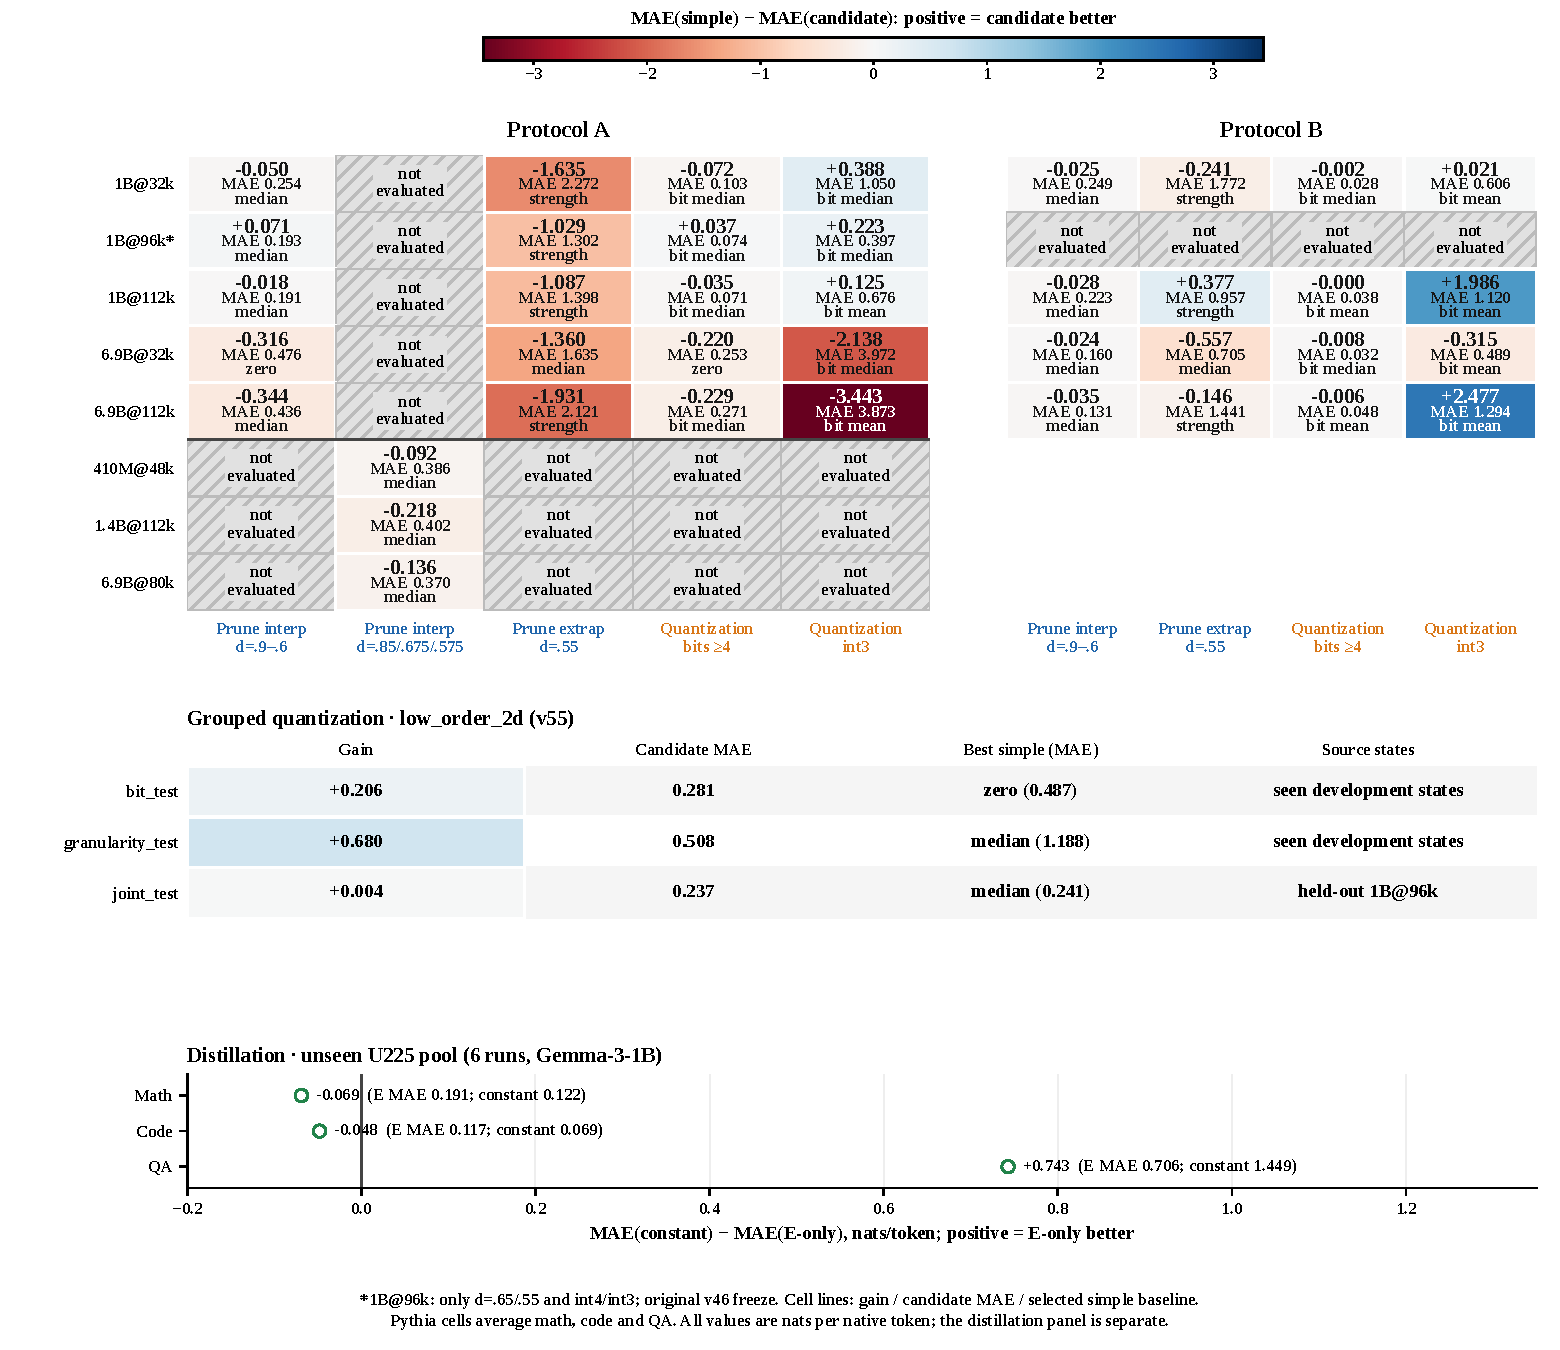
\includegraphics[width=0.7\textwidth]{figs/transfer_limits.pdf}
\caption{Generalization to unseen configurations and states. Top: improvement of the headline candidate over the strongest source-free reference (MAE difference, nats, averaged over the three capabilities; positive = candidate better) for each new source (rows), regime (columns), and fitting protocol (panels), with the candidate MAE printed in each cell; the confirmation panel (410M@48k, 1.4B@112k, 6.9B@80k) and the grouped-quantization tests are included. Cells not evaluated are hatched. Bottom: the distillation pool tests, per capability, against the frozen constant. All predictions were frozen before the corresponding measurement.}
\label{fig:transfer}
\end{figure}
\subsection{Prediction at Unseen Compression Settings}
\label{sec:unseen_settings}

\paragraph{Pruning densities.} On the three checkpoints that entered
no fit, at densities 0.85, 0.675, and 0.575, the delivered power form
has MAE 0.24, 0.24, and 0.68 for math, code, and QA: it beats the
strength-only curve (0.45, 0.49, 0.58) and zero change on every
checkpoint, has the lowest math error of all predictors, ties the
median curve on code, and loses QA to every source-free curve (median
0.22) because it over-predicts the QA improvement, so the median has
the lowest aggregate error (0.24 against 0.39). At $d=0.55$, beyond
the range, every source-conditioned form fails on every source (0.6
to 4.5 nats): the transfer range is the interpolation regime.

\paragraph{Quantization settings.} The per-channel predictor's one
unseen setting, 5 bits by a fixed interpolation rule, is worse than a
per-bit constant on the 1B source. With group size as a second axis,
the frozen surface of Eq.~\eqref{eq:quant2d} has MAE 0.19, 0.21, and
0.44 at the unseen $b=4$ on the six development states (zero change
0.45, 0.53, 0.48; per-configuration median 0.55, 0.73, 0.54) and
0.22, 0.32, 0.99 at the unseen $g=128$ across three bit-widths (zero
change 1.24, 1.35, 1.24). The separable power candidate we tested is
worse than zero change on the bit test and the bilinear interpolation
fails outside the development corners; other amplitude-times-shape
forms remain untested. On the one new state tested (1B@96k at
$g=128$, three cells) the surface is best on code and behind the
source-free curves on math and QA.

\paragraph{Distillation pools.} On the earlier protocol, the
reuse-count form frozen on pools U75 and U600 beats the constant on
the unseen pool U225 only for QA (0.706 against 1.449), with a bias
that changes sign across budgets, and variation across pool samples
exceeds variation across training seeds (0.43 against 0.04 nats;
under the uniform protocol two seed repeats differ from their
originals by at most 0.03 nats for math and code and 0.19 for QA at
the largest reuse count, Appendix~\ref{sec:app_results}). Under the
uniform protocol, the headline joint form beats the frozen
per-capability constant on every capability of both development
students at the unseen pool (math 0.045 and 0.050 against 0.060 and
0.057; code 0.036 and 0.029 against 0.047 and 0.069; QA 0.61 and 0.44
against 0.86 and 1.00; Table~\ref{tab:p2v2_test}), so the pool
direction is covered on the development students.

\subsection{Transfer across Model Sizes and Training Stages}
\label{sec:unseen_states}

Inside the range, the frozen per-density pruning regression beat its
no-$D_0$ variant and the per-setting median on all three capabilities
at the unseen stage 96k for the 160M and 1.4B sources, and for a 1B
source at steps 32k and 112k the power form, A2, and the median curve
are within 0.05 nats of one another, so a new in-range size is
predicted about as well by the source relation as by the development
median. For a 6.9B source, five times the development range, the
source-conditioned pruning forms lose to the median curve on math
(0.30 against 0.12) and QA (0.91 against 0.12) and tie on code: the
regression extends the panel's size trend into QA improvements that
do not occur, and the per-bit quantization regression is worse than
the per-bit median at every bit-width. On 6.9B@80k the power form
ties the median on math (0.30 against 0.31) and loses on code and QA:
the size boundary is soft for math and hard for QA. For distillation,
on Gemma-3-4B as a held-out student ($\log N_S$ 1.9 above the
reference against a development span of $\pm0.55$) the headline form
loses to the frozen constant at the unseen pool (math 0.089 against
0.020, code 0.050 against 0.038, QA 1.14 against 1.02), because its
source term extends the QA reuse penalty to 2.3 nats at the largest
budget where 0.40 was measured, and beats the constant at the
development pools (0.106, 0.048, 0.96 against 0.156, 0.098, 1.79;
Table~\ref{tab:p2v2_test}). Joint transfer to a larger student and a
new pool remains unreliable.

\subsection{Applicability across Capabilities and Shared Structure}
\label{sec:capabilities}

Math and code are carried by the initial-state inputs on every axis,
QA is not: its pruning response is over-predicted by every
source-conditioned form on every new checkpoint, and its quantization
error is the largest of the three on every test. Conditioning is also
needed in the response shape: per-capability distillation models at
the same parameter count as a shared-shape model lower the held-out
error by 0.1 to 0.4 nats for the budget-plus-reuse structures
(Appendix~\ref{sec:app_forms}, Fig.~\ref{fig:inputs}).

\paragraph{Shared structure, ranges, and calibration.} One function
family for all three methods, with method- and capability-specific
parameters, holds for pruning by construction and fails for the other
two arms on the same held-out splits (the separable family we tested
is worse than the quantization surface, macro MAE 2.96 against 2.40;
a reuse-only family is worse than the budget-plus-reuse form, 0.54
against 0.28). Within pruning one exponent shared across capabilities
costs nothing (leave-one-source MAE 0.351, 0.338, 0.785 against 0.328,
0.355, 0.798), whereas the quantization coefficients must be
capability-specific. Three ranges are kept apart
(Appendix~\ref{sec:app_shared}): the bootstrap intervals of the
pruning coefficients exclude zero for the dense-anchor term on math
and code and not on QA; exponents fitted per source spread from 3.0
to 6.0 for math and 0.5 to 6.0 for QA; and 80\% prediction intervals
from leave-one-source residuals under-cover, at 78\% on the 27
confirmation-panel cells and 67\% on the 1B and 6.9B pair cells, with
a mean full width near 1.5 nats, which we report as such. One
measured calibration point helps or hurts by method: setting the
pruning amplitude from the target's mildest density amplifies noise
through the steep exponent (leave-one-source MAE above 17 nats),
whereas a separable grouped-quantization law calibrated at the single
5-bit, $g=256$ cell predicts the unseen 4-bit configurations on
held-out states with MAE 0.13, 0.12, 0.29 against 0.26, 0.64, 1.34
uncalibrated, at the cost of one compressed measurement per source.

\FloatBarrier
